\newcommand{\loft}[5]{\ensuremath{\textcolor{magenta}{\Omega{\bf \mathcal{L}}_{#1}^{#2,#3}}[\textcolor{blue}{\{#4\}}\textcolor{red}{(#5)}]}}

\newcommand{\affine}[5]{\ensuremath{\textcolor{magenta}{\Delta{\bf \mathcal{A}}_{#1}^{#2,#3}} [\textcolor{blue}{\{#4\}} \textcolor{red}{(#5)}]}}

\newcommand{\boolop}[5]{\ensuremath{\textcolor{magenta}{\Omega{\bf \mathcal{B}}_{#1}^{#2,#3}}[\textcolor{blue}{\{#4\}} \textcolor{red}{(#5)}]}}

\newcommand{\generic}[7]{\ensuremath{\textcolor{magenta}{#1{\bf \mathcal{#2}}_{#3}^{#4,#5}}[\textcolor{blue}{\{#6\}} \textcolor{red}{(#7)}]}}
\newtheorem{mydef}{Definition}
\newtheorem{mylem}{Remark}

\section{Proposed Approach}
\label{sec:approach}
Following section provides an overview of the system and the overall work-flow:

\bigskip

\begin{minipage}[c]{0.98\linewidth}
    \begin{minipage}[c]{0.57\linewidth}
\begin{itemize}[noitemsep,topsep=2pt,parsep=2pt,partopsep=2pt,leftmargin=*]
\item \textbf{Input}: Feature-based CAD models, which are widely available in most of the commercial CAD applications. It is represented by  ($\cup_qf^3$), where `$\cup$' denotes a collection, of `$q$' features (`$f$') having dimensionality `$3$' (solids). Thin-walled CAD models come in various representations, such as mesh, solid, feature-based, etc. This research expects a feature-based CAD model, which can be deemed as limitation in case of its unavailability. But, techniques, such as segmentation, decomposition, feature recognition (FR), etc. can convert a non-feature-based representation to the feature-based CAD model.

\item \textbf{Defeaturing}:  Computes gross shape by removing irrelevant/superficial features. It has two approaches - first, sheet metal features are classified into suppressible and non-suppressible features, based on the newly-proposed taxonomy and the second, a generic technique based on geometric reasoning is proposed to identify the suppressible features. Defeatured model  is denoted as ($\cup_rf^3, r \leq q$).%  (\cite{YogeshCADConf2015}). 

\item \textbf{Generalization}: As mentioned in Section \ref{sec:facepairdetection} ``ABEL'' transforms form-features to ``Loft/Sweep'' representations ($L$), making it simpler to develop further algorithms as one does not need to consider specifics of a plethora of form feature types. The model thus becomes ($\cup_rL^3$).%  (\cite{YogeshIITG2014}). 

\item \textbf{Decomposition}: Cellular decomposition is performed at each Loft/Sweep feature step to form non-volumetrically-overlapping cellular bodies having respective owner-Sweep/Loft feature. A cellular-graph is populated with the cellular bodies at the graph-nodes and face-interfaces as edges.

\item \textbf{Midsurface Computation}: Using topology of the graph, the nodes are classified into midsurface-patch generating nodes (solid cells - $sCell$s) and interaction-resolving nodes (interface cells - $iCell$s). 

\item \textbf{Validation}:  Midsurface needs to faithfully mimic the parent shape. A topological method is proposed and used to validate correctness of the midsurface.

\item \textbf{Output}: A well-connected midsurface is then sent to downstream applications such as CAE analysis.
\end{itemize}

    \end{minipage}
    \hfill
    \begin{minipage}[c]{0.4\linewidth}
	\centering 
	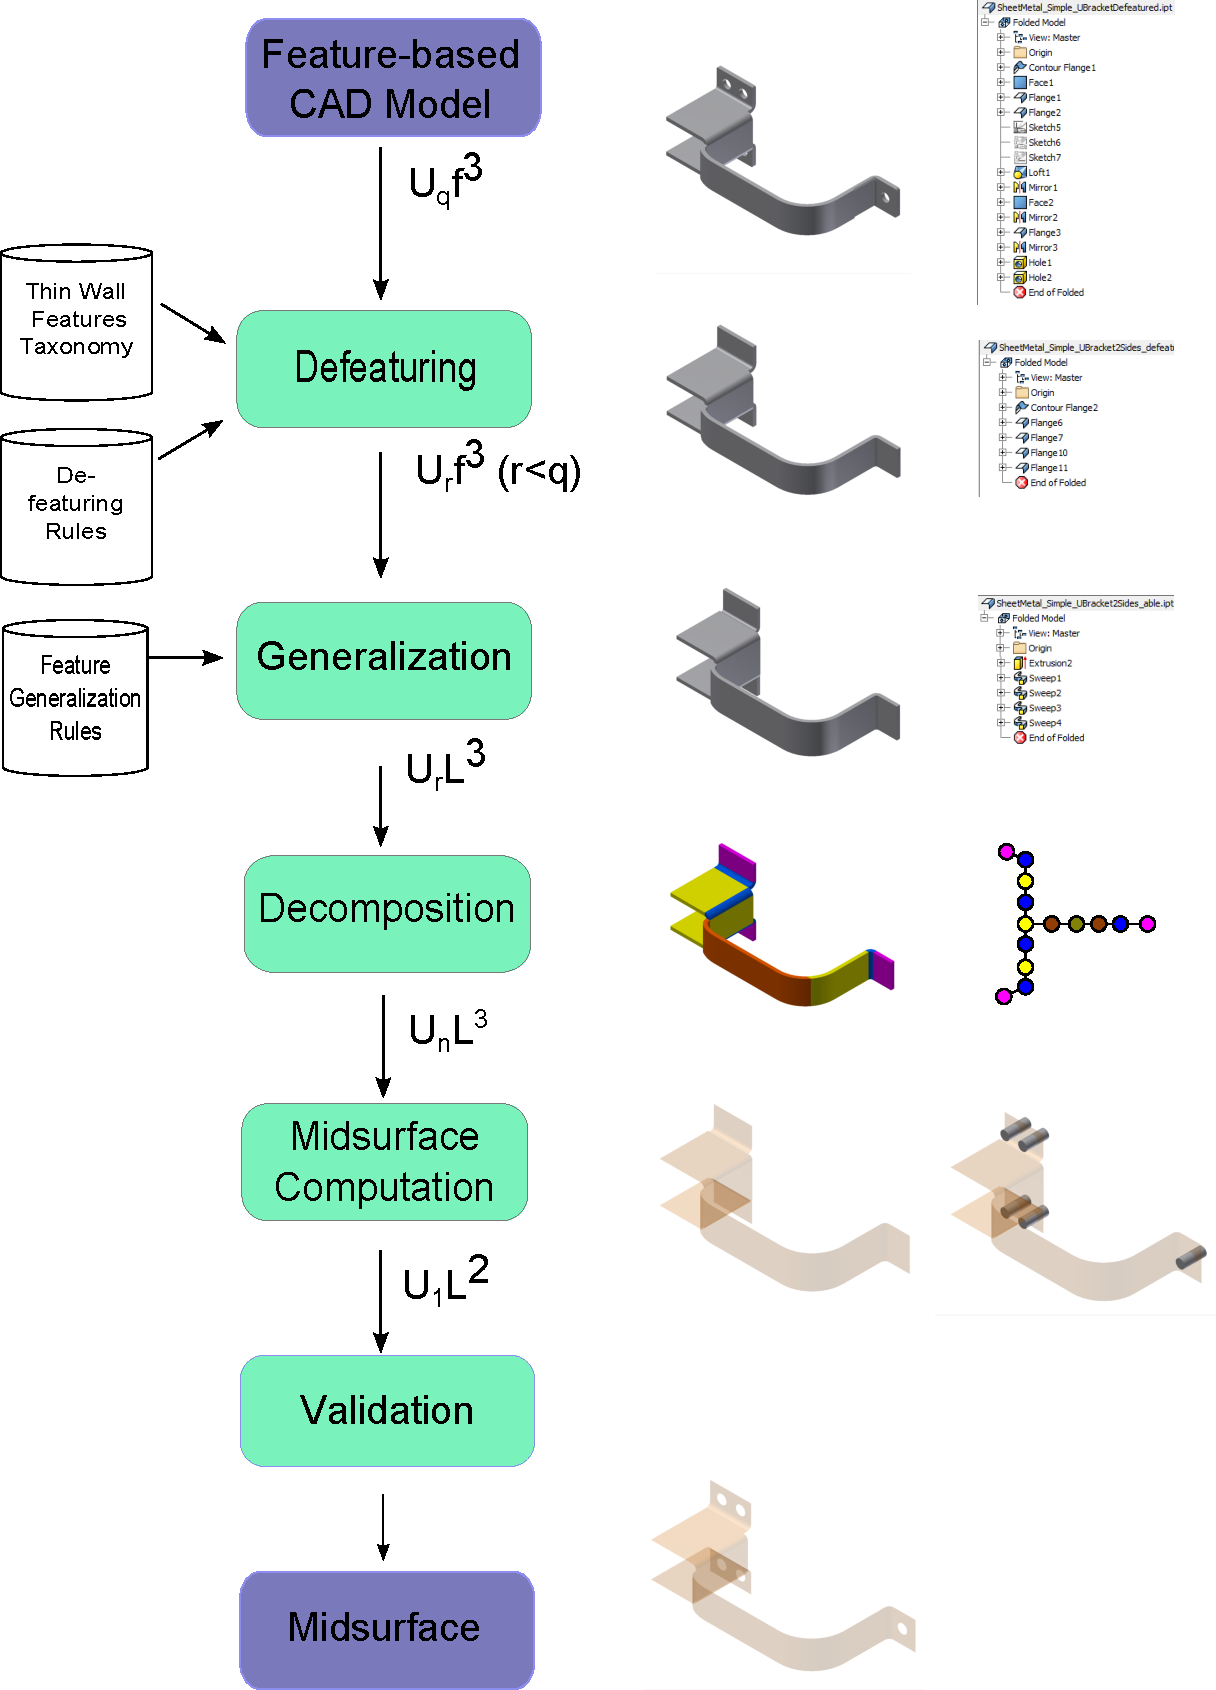
\includegraphics[width=0.95\linewidth]{../Common/images/SystemArchitecture3.pdf}
	\captionof{figure}{Overall work-flow}
	\label{fig_sysarch}
    \end{minipage}

\end{minipage}    

\bigskip

Following sections provide details of each of the above-mentioned modules.

\section{Defeaturing}
It has been observed that a simplified shape which retains the overall shape, called ``gross shape'', yields more effective midsurface. Thus, the objective of this defeaturing module is to compute the gross shape by removing irrelevant features. The selection/eligibility of the irrelevant features is decided by two proposed approaches. In the first, which is sheet metal domain-specific, a newly proposed taxonomy (Figure \ref{fig:tax_sm}) is used for decision of suppressibility. In the second, a generic technique based on geometric reasoning is proposed to identify the suppressible features. These approaches are implemented as phases I and II and come sequentially one after another. Further, both phases can be customized. Phase I can be customized for different domains by providing respective taxonomy of that domain. Phase II can be customized with different size-threshold values.

\subsection{Phase I: Defeaturing based on the application context (Sheet Metal)}\label{ph1}
Proposed  taxonomy (Figure ~\ref{fig:tax_sm}) is used to decide suppressibility of a sheet metal feature.

\begin{minipage}[c]{0.98\linewidth}
\begin{minipage}[t]{0.5\linewidth}
\begin{itemize}
[noitemsep,topsep=2pt,parsep=2pt,partopsep=2pt]
\item \textbf{Primary Features}: These are not suppressed irrespective of their size as they form the principal/gross shape.  Their absence will create missing midsurface patches. Examples:
	\begin{itemize} [noitemsep,topsep=2pt,parsep=2pt,partopsep=2pt]
	\item Face-Wall
	\item Flange
	\item Drawing
	\end{itemize}
\item \textbf{Secondary Features}: These are suppressed based on their relative smaller size with respect to the overall input-shape and the size-threshold. 
 Examples:
	\begin{itemize} [noitemsep,topsep=2pt,parsep=2pt,partopsep=2pt]
	\item Stamping
	\item Emboss 
	\end{itemize}
	
\item \textbf{Tertiary/Auxiliary Features}: They are helper/ancillary shapes and thus, not a part of the gross/overall shape. So they can be suppressed irrespective of their sizes.
Examples:
	\begin{itemize} [noitemsep,topsep=2pt,parsep=2pt,partopsep=2pt]
	\item Lip
	\item Rest 
	\end{itemize}
	
%\item \textbf{Connecting Features}: These are not suppressed irrespective of their sizes, as removing them, will create gaps between the sub-shapes of the original part. Lacking these would create gaps, so these are retained irrespective of their relative size, small or large.
%Example is:
%	\begin{itemize} [noitemsep,topsep=2pt,parsep=2pt,partopsep=2pt]
%	\item Bend
%	\end{itemize}
		
\item \textbf{Feature Groups}: These are feature collections. Their suppressibility is evaluated as a collection with the size-based criterion. 	Examples:
\begin{itemize} [noitemsep,topsep=2pt,parsep=2pt,partopsep=2pt]
	\item Mirror
	\item Patterns
	\end{itemize}
\end{itemize}

\end{minipage}
\hfill
\begin{minipage}[t]{0.48\linewidth}
\begin{minipage}[t]{\linewidth}
\dirtree{%
.1 Sheet Metal Features.
.2 Primary Features.
.3 Face-Wall   \adjustbox{valign=t}{
\includegraphics[scale=0.65]{..//Common/images/InventorWall.png}}.
.3 Flange  \quad \adjustbox{valign=t}{
\includegraphics[scale=0.65]{..//Common/images/InventorFlange.png}}.
.3 Bend   \qquad \adjustbox{valign=t}{
\includegraphics[scale=0.65]{..//Common/images/InventorBend.png}}.
%.3 Loft Flange  \qquad \adjustbox{valign=t}{
\includegraphics[scale=0.65]{..//Common/images/InventorLoftedFlange.png}}.
%.3 Rib \quad \quad  \adjustbox{valign=t}{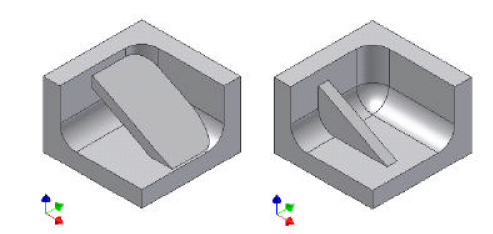
\includegraphics[height=0.11\linewidth]{..//Common/images/Feature_Rib.png}}.
.2 Secondary Features.
.3 Stamping  \quad \adjustbox{valign=t}{
\includegraphics[scale=0.65]{..//Common/images/InventorStamping.png}}.
.3 Cutout  \qquad \adjustbox{valign=t}{
\includegraphics[scale=0.65]{..//Common/images/InventorCutout.png}}.
%.3 Fold  \qquad \adjustbox{valign=t}{
\includegraphics[scale=0.65]{..//Common/images/InventorFold.png}}.
%.3 Roll  \qquad \adjustbox{valign=t}{
\includegraphics[scale=0.65]{..//Common/images/InventorRoll.png}}.
.3 Emboss \qquad \adjustbox{valign=t}{
\includegraphics[scale=0.65]{..//Common/images/InventorEmboss.png}}.
%.3 Hem   \quad \qquad \adjustbox{valign=t}{
\includegraphics[scale=0.65]{..//Common/images/InventorHem.png}}.
%.3 Grill \qquad \adjustbox{valign=t}{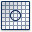
\includegraphics[scale=0.65]{..//Common/images/InventorGrill.png}}.
.2 Tertiary/Auxiliary Features.
%.3 Chamfer \qquad \adjustbox{valign=t}{
\includegraphics[scale=0.65]{..//Common/images/InventorChamfer.png}}.
%.3 Round  \qquad \adjustbox{valign=t}{
\includegraphics[scale=0.65]{..//Common/images/InventorRound.png}}.
%.3 Thread \qquad \adjustbox{valign=t}{
\includegraphics[scale=0.65]{..//Common/images/InventorThread.png}}.
.3 Lip \qquad \adjustbox{valign=t}{
\includegraphics[scale=0.65]{..//Common/images/InventorLip.png}}.
.3 Rest \qquad \adjustbox{valign=t}{
\includegraphics[scale=0.65]{..//Common/images/InventorRest.png}}.
%.2 Connecting Features.
%.3 Bend   \qquad \adjustbox{valign=t}{
\includegraphics[scale=0.65]{..//Common/images/InventorBend.png}}.
.2 Features Groups.
.3 Mirror \quad  \quad \adjustbox{valign=t}{
\includegraphics[scale=0.65]{..//Common/images/InventorMirror.png}}.
%.3 RectPattern \quad  \adjustbox{valign=t}{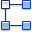
\includegraphics[scale=0.65]{..//Common/images/InventorRectPattern.png}}.
.3 Pattern\quad  \adjustbox{valign=t}{
\includegraphics[scale=0.65]{..//Common/images/InventorCircPattern.png}}.
}
\captionof{figure}{Sheet Metal features taxonomy (Icons source: \cite{Inventor2014Help})}\label{fig:tax_sm}
\end{minipage}
\end{minipage}
\end{minipage}    

\smallskip

The Phase I process is shown pictorially below. The first picture of Fig. \ref{fig:phaseI}

\smallskip

\begin{minipage}[t]{\linewidth}
\begin{tabular}[h]{@{} p{0.3\linewidth} p{0.3\linewidth}  p{0.3\linewidth}@{}} \toprule

\textbf{Input model to Phase I} & \textbf{Selected sheet metal features} & \textbf{Output of Phase I} \\ \midrule

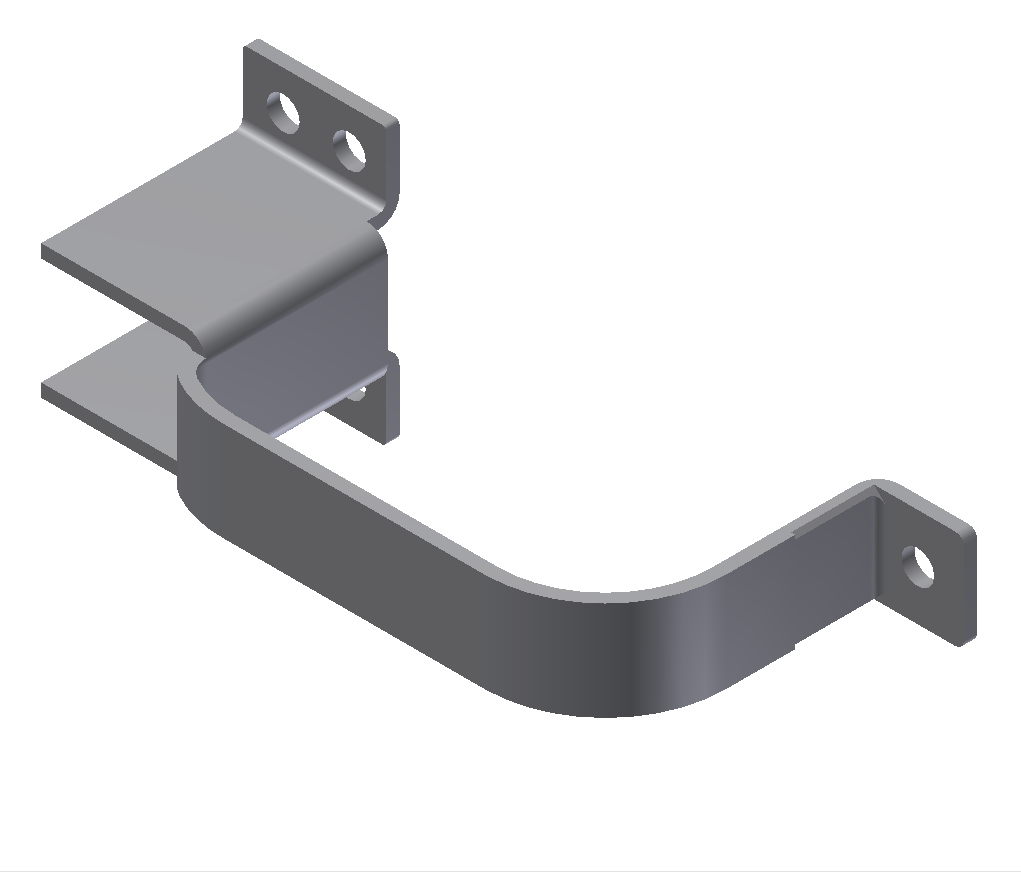
\includegraphics[width=0.98\linewidth]{..//Common/images/DefeatBracketPhase_I_1} &
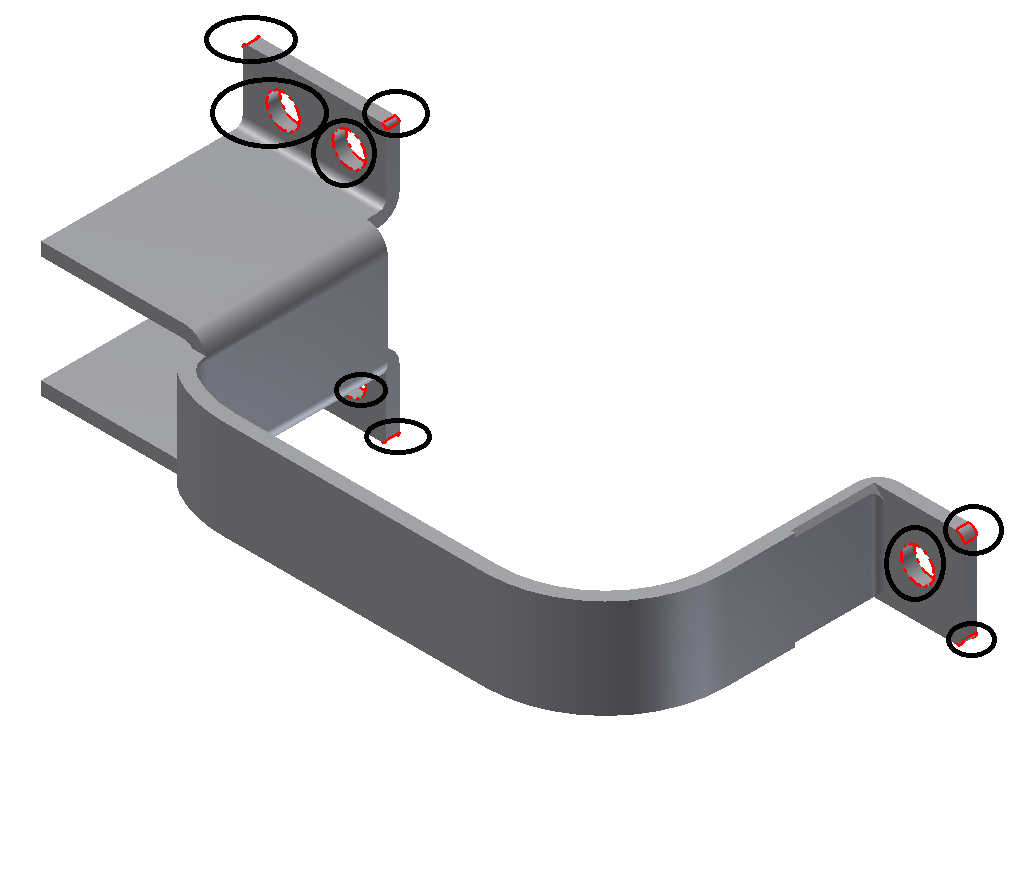
\includegraphics[width=0.98\linewidth]{..//Common/images/DefeatBracketPhase_I_2_circled} &
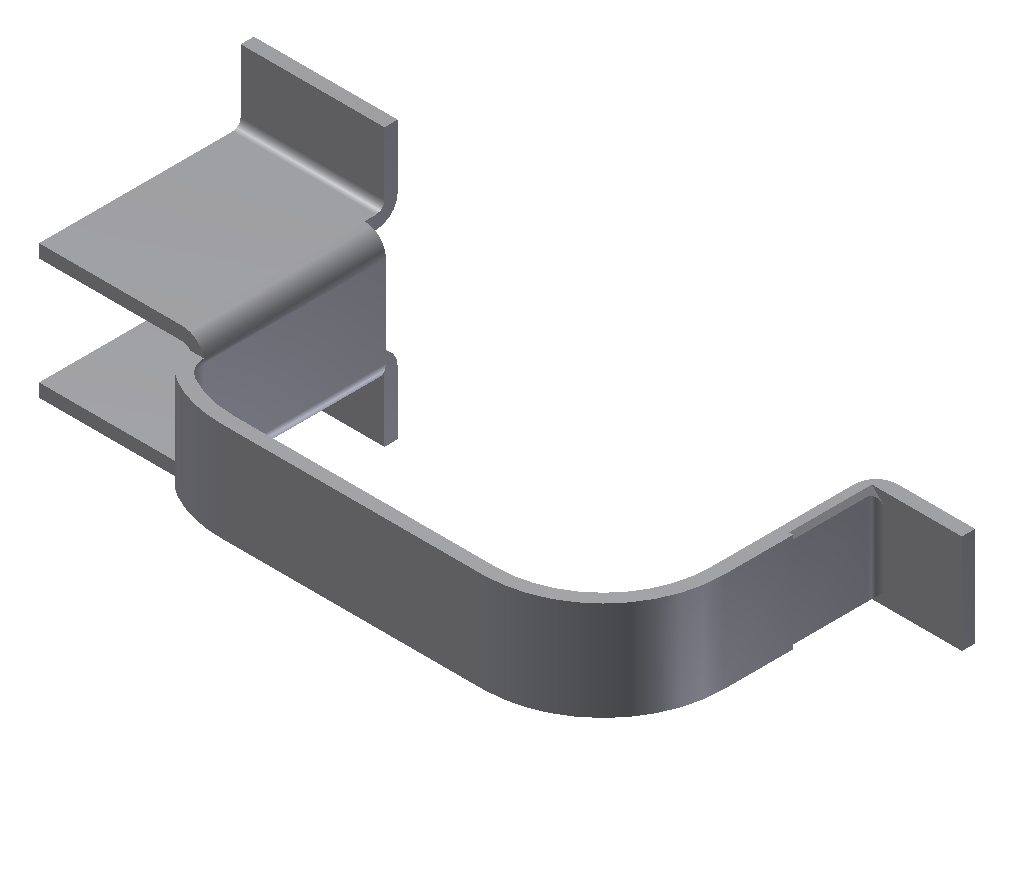
\includegraphics[width=0.98\linewidth]{..//Common/images/DefeatBracketPhase_I_3} \\ \bottomrule

\end{tabular}
\captionof{figure}{Phase I: Defeaturing based on the application context (Sheet Metal)}\label{fig:phaseI}
\end{minipage}

\subsection{Phase II: Defeaturing based on Geometric Reasoning} \label{ph2}

In the feature-based design paradigm, the CAD model is built step by step using features at each step. Feature parameters are used to compute the ``canonical'' (tool-body) volume first, which is then booleaned to the model built till then. During this operation, some portion of the canonical volume may get consumed, leaving behind the remaining (remnant) volume in the final solid  (Fig.~\ref{fig_remnant}). Identification of suppressible features based on the feature volume computed from the full feature parameters yield incorrect results as the final shape may not retain the full feature volume. So, this work has devised a novel technique  to find the size of remnant feature volume to be used for deciding the suppressibility  (Fig.~\ref{fig:phaseII}) of the features.

\begin{minipage}{0.98\linewidth}
	\begin{minipage}[b]{0.28\linewidth}
	 \raisebox{-.9\height}{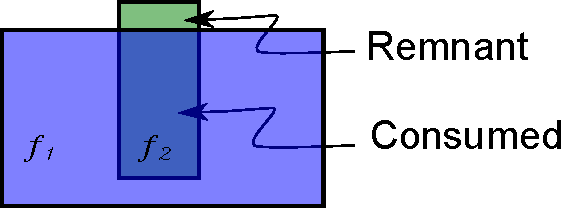
\includegraphics[width=\linewidth]{../Common/images/Solid_Simple_SmallProtrusion.pdf}}
	 \captionof{figure}{Remnant and Consumed}
	 \label{fig_remnant}
	\end{minipage}
\hfill
	\begin{minipage}[b]{0.3\linewidth}
	\raisebox{-.9\height}{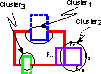
\includegraphics[width=0.8\linewidth]{../Common/images/clusters.pdf}}
	\captionof{figure}{Formation of clusters} \label{fig_clusters}
	\end{minipage}
\hfill
	\begin{minipage}[b]{0.3\linewidth}
	\raisebox{.9\height}{
	\begin{tabular}[h]{@{} p{0.3\linewidth} p{0.3\linewidth} p{0.3\linewidth}@{}} \toprule
	\textbf{Clusters} & \textbf{Size}& \textbf{Feature}\\ \midrule
	cluster$_1$ & 0.25 	&  Extrude$_2$\\
	cluster$_2$ & 0.25  & Extrude$_3$\\
	cluster$_3$ & 0.125 & Hole$_1$\\ \bottomrule
	%$f_{10}, f_{12}, f_{15}, f_{14}$ 	& Cluster$_4$\\ \bottomrule
	\captionof{table}{ Clusters}
	\label{tbl_clusters}
	\end{tabular}
	}
	\end{minipage}
\end{minipage}

Algorithm to identify candidate features for de-featuring based on Remnant Feature method:
\begin{itemize}
[noitemsep,topsep=2pt,parsep=2pt,partopsep=2pt]
\item Faces of the final body are iterated. 
\item For each remnant face, its owning feature is extracted via attributes stored on them. 
\item Clusters/Groups of faces are built based on the owning features as shown in Fig. \ref{fig_clusters}. The dotted portion in a cluster represents the Consumed Feature, whereas the encircled portion is the Remnant feature
\item Size of the cluster can be calculated by various techniques like Influence Volume (obtained as a difference of the volume, if the feature is suppressed and then unsuppressed) or the union of bounding-boxes, etc. This work uses summation of the area of the remnant faces (Tab. \ref{tbl_clusters}) as per the Size criterion.
\item Each cluster-owning feature(s) is added to {\em sl} based on the threshold value given by the user.
\item The {\em sl}  is presented to the user for verification and changed, if necessary. 
\item Features in {\em sl} are suppressed.
\end{itemize} 

\begin{minipage}[t]{\linewidth}
\begin{tabular}[h]{@{} p{0.3\linewidth} p{0.3\linewidth}  p{0.3\linewidth}@{}} \toprule

\textbf{Input model to Phase II} & \textbf{Selected Remnant method} & \textbf{Output of Phase II} \\ \midrule


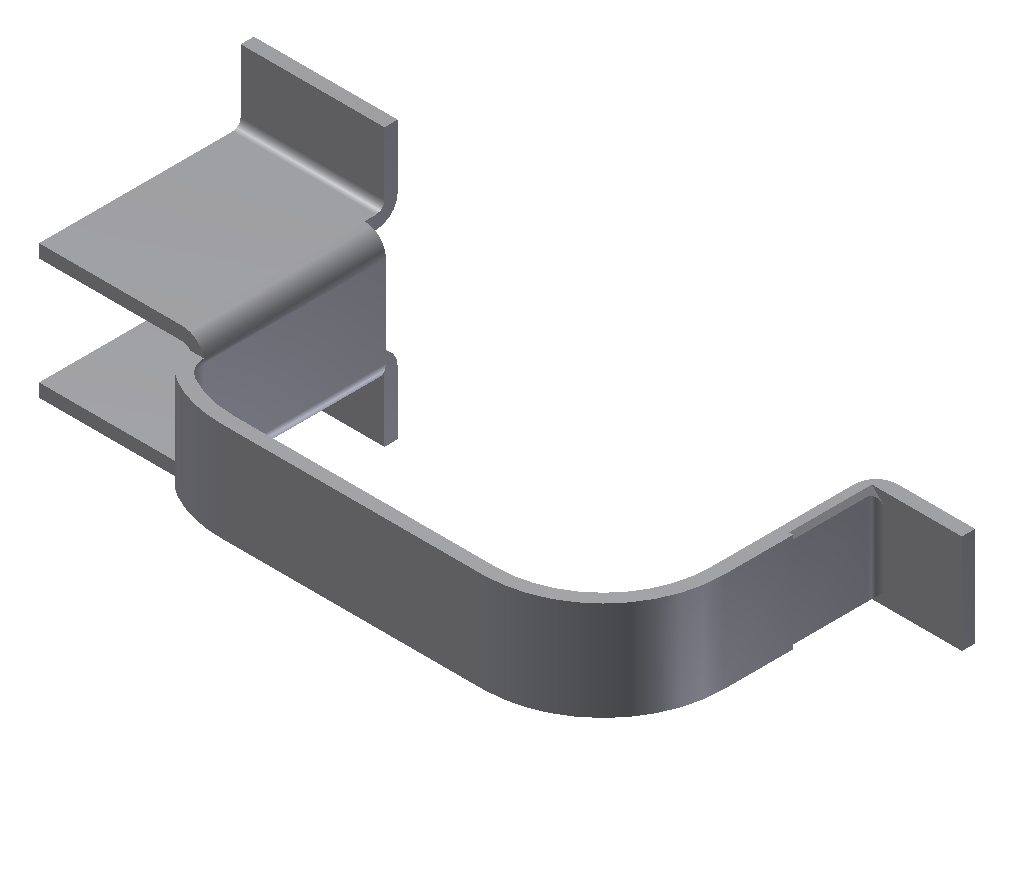
\includegraphics[width=0.98\linewidth]{..//Common/images/DefeatBracketPhase_I_3} &
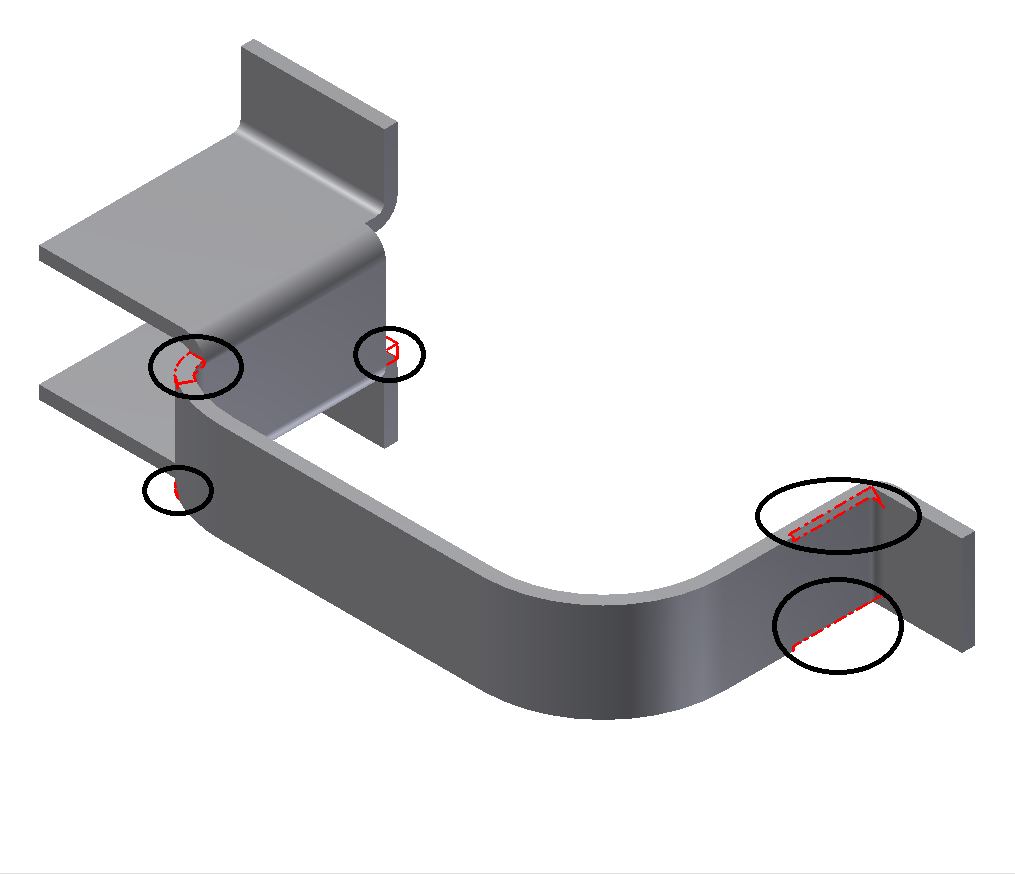
\includegraphics[width=0.98\linewidth]{..//Common/images/DefeatBracketPhase_II_2_circled} &
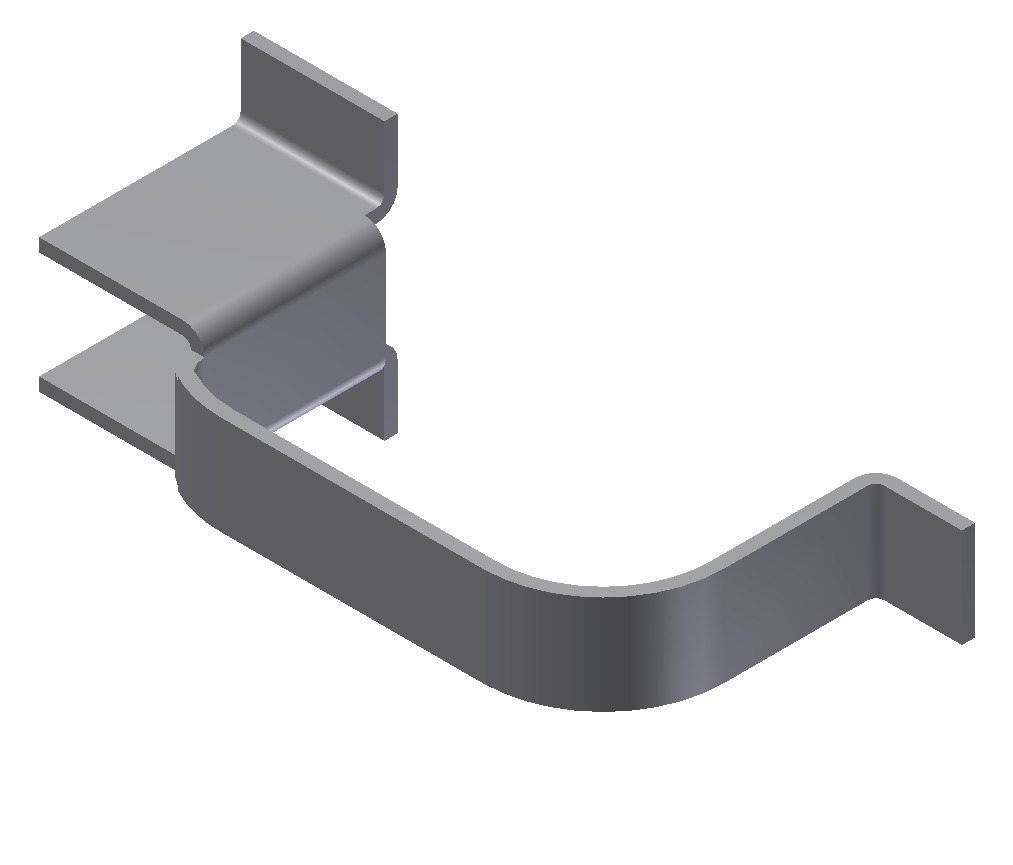
\includegraphics[width=0.98\linewidth]{..//Common/images/DefeatBracketPhase_II_3} \\ \bottomrule

\end{tabular}
\captionof{figure}{Phase II: Defeaturing based on Geometric Reasoning}\label{fig:phaseII}
\end{minipage}

Output of Phase II (Fig. \ref{fig:phaseII}) is the gross shape of the input given (Fig. \ref{fig:phaseI}). With 50\% reduction in the number of features and 17\% reduction in the number of faces, the gross shape resulted has retained all the important features necessary for the computation of a well-connected midsurface.

\subsection{Dormant Feature-Bodies}\label{sec:dormant}

In addition to the phases mentioned above, a novel idea of caching large/relevant negative features is used.  Large/relevant but negative features, like Holes, Cut, which by usual rules would not get suppressed, are suppressed and their tool/canonical body is preserved. These bodies, called ``Dormant bodies'', are then used to pierce the final midsurface. With this novel arrangement, computing midsurface patches is simplified due to lack of holes, while re-piercing of the cached dormant bodies ensures their faithful representation in the midsurface.


\section{Abstraction/Generalization}
In the Generalization/Abstraction module, input feature tree is converted into Loft/Sweep/Extrude/Revolve tree (Figure \ref{fig:abel}) . This abstracted tree is then sent for Midsurface computation. 

\subsection{Notation}
A generic notation scheme is developed to represent various CAD entities/operations. It is loosely based upon Interactive Configuration Exploration  (ICE) scheme developed by Moustapha \cite{Hoda2005} for architectural applications. Although some of the fundamental entities and syntax are borrowed from ICE, it has been further enhanced to suit Mechanical CAD applications.  Once the model is represented in terms of ICE entities, further transformations/algorithms can be written on top using the same notations. In the context of current research, it is shown that most of the form features can be represented as Loft/Sweep feature notation and then midsurface transformation is developed on the Loft/Sweep(and internal booleans) only, thus making the algorithm generic. In ICE, a generic {\em Operator/Regulator} is represented as \\

{\generic{category}{R}{instance}{subtype}{dimension}{arguments}{shapes}}\\

	 For example ,

	\affine{}{T}{1}{\bar{p},line,n}{shape} 
	
	where,
		\begin{itemize}[noitemsep,topsep=0pt,parsep=0pt,partopsep=0pt,label={}]
		\item 	\textcolor{magenta}{$\Delta$} : Transformation category (type)
	     	\item 	\textcolor{magenta}{${\bf \mathcal{A}}$} : Affine Transformation regulator (type)
		\item  	\textcolor{magenta}{$^T$}: subtype Translation (type)
		 \item 	\textcolor{magenta}{$^1$} : dimensionality of output (integer)
	        \item 	\textcolor{blue}{ $\bar{p}$} : position (point)
  		\item  	\textcolor{blue}{$line$} : linear guide (curve)
		 \item  	\textcolor{blue}{$n$} : number used for copies, scaling, etc. (float)
		 \item  	\textcolor{red}{$shape$} : target (shape)
		\end{itemize}

Most of the form feature used in CAD applications can be modeled using  three Regulators: Affine Transformation ($\mathcal{A}$),  Boolean ($\mathcal{B}$) and Loft ($\mathcal{L}$), while  operating on the Entities($\mathcal{E}$).  This representation is called as {\bf $\mathcal{ABLE}$}. 

\subsection{Abstract Loft/Sweep}

Loft is a generic operator (Figure \ref{figure_Loft})  capable of generating most of the basic shapes. It joins {\em profiles} along a guide {\em curve}.  Sweep is a specialized case of Loft (with a single profile and a singe guide curve). Sweep and Loft, though distinct, are used interchangeably in the context of constant thickness thin-walled solids.

\begin{minipage}{0.98\linewidth}
	\begin{minipage}[c]{0.4\linewidth}

%\begin{tabular}{  p{0.22\textwidth}  p{0.22\textwidth} }

	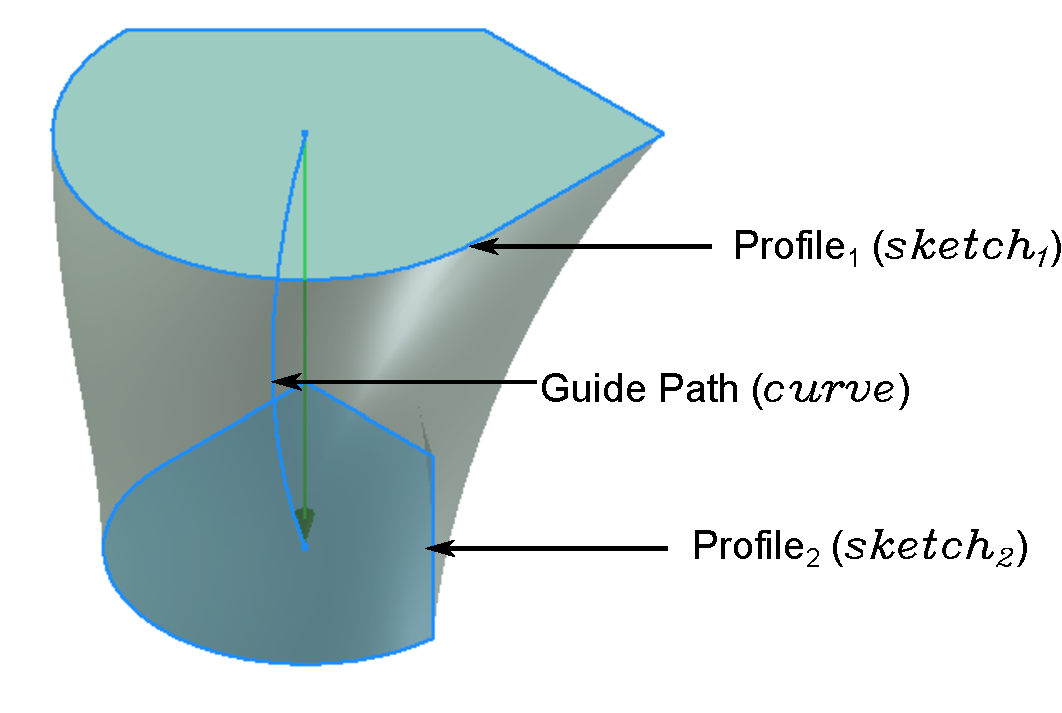
\includegraphics[scale=0.35]{../Common/images//LoftPreview.pdf} 
	%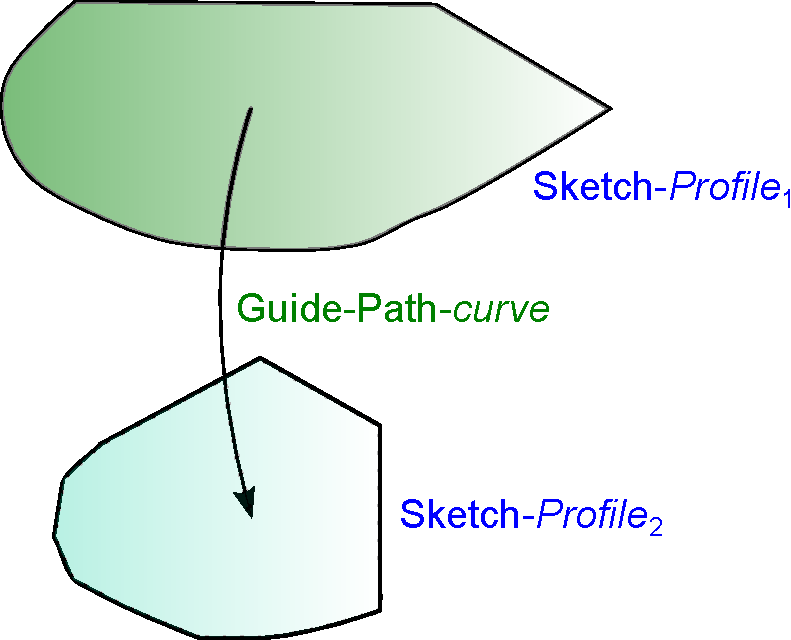
\includegraphics[scale=0.3]{../Common/images//LoftProfilesPath.pdf} \\

%\end{tabular}
\captionof{figure}{Generic Loft feature}
\label{figure_Loft}


	\end{minipage}
\hfill
	\begin{minipage}[c]{0.52\linewidth}
	Represented as:
	\vskip 2mm
	\loft{}{subtype}{3}{0, curve, 0 | C_{0,1,2}}{ (sketch )^{<1-n>}}
	\vskip 2mm
	
	{\em Continuity} options like $C_0$ for connectedness, $C_1$ for tangency and $C_2$ for curvature continuity can be specified at the ends where the body generated by the {\em Loft} joins the existing shape. In case this body is disjoint or is the first one in the scene, no {\em continuity}  is specified. Some form features also specify a {\em draft-angle}  for tapering sides. This can be modeled as {\em Loft} between two {\em profiles}, where the second {\em profile} is offset-ed inside or outside. Output of the Loft can either be a $solid$ (where capping faces are added to close the shape) or a $surface$ (capping faces are not added) and accordingly, dimensionality of $2|3$ can be specified.

	\end{minipage}
\end{minipage}


\bigskip

\begin{minipage}[t]{\linewidth}
\begin{tabular}[h]{@{} p{0.24\linewidth} p{0.22\linewidth} |  p{0.24\linewidth}  p{0.22\linewidth}@{}} \toprule

\textbf{Input Tree} & \textbf{Input Model} & \textbf{Output Tree} & \textbf{Output Model}\\ \midrule


\raisebox{-.9\height}{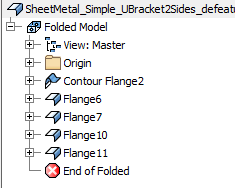
\includegraphics[width=0.98\linewidth]{..//Common/images/ABELBracketInputTree}}&
\raisebox{-.9\height}{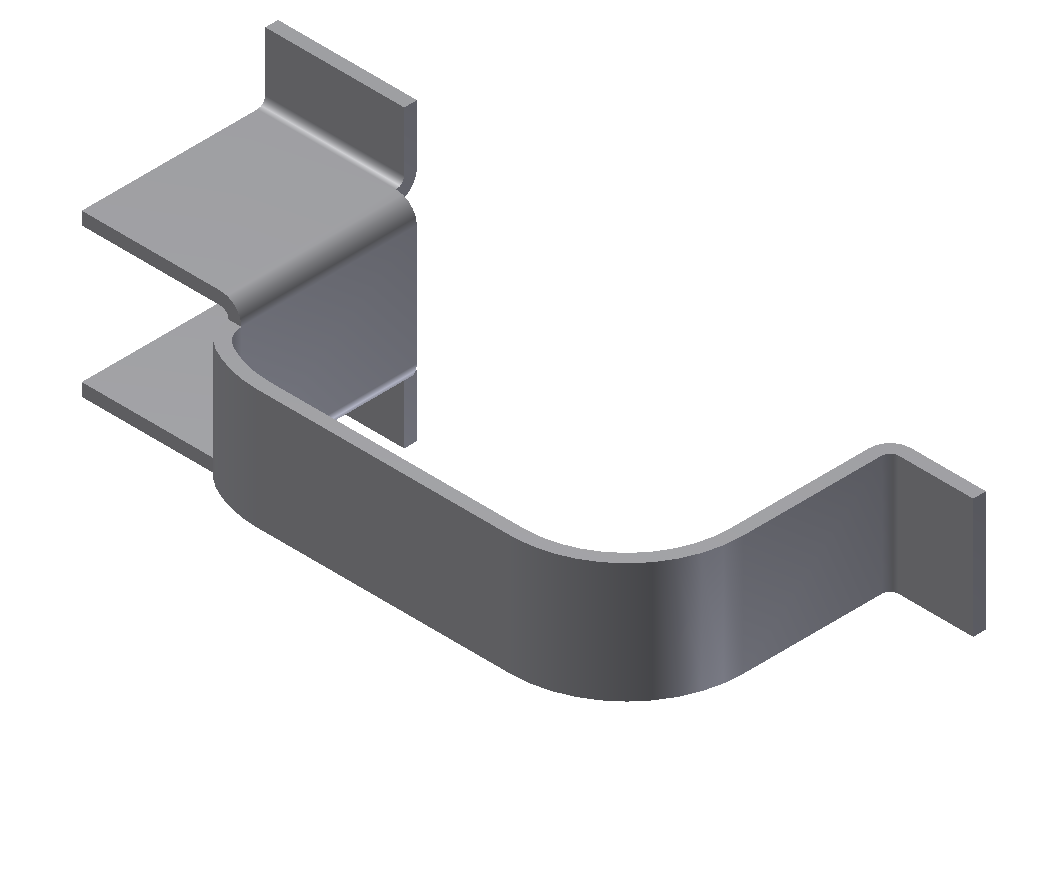
\includegraphics[width=0.98\linewidth]{..//Common/images/ABELBracketInputPart}} &
\raisebox{-.9\height}{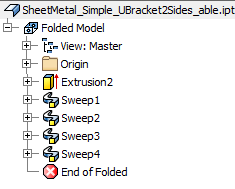
\includegraphics[width=0.98\linewidth]{..//Common/images/ABELBracketOutputTree}} &
\raisebox{-.9\height}{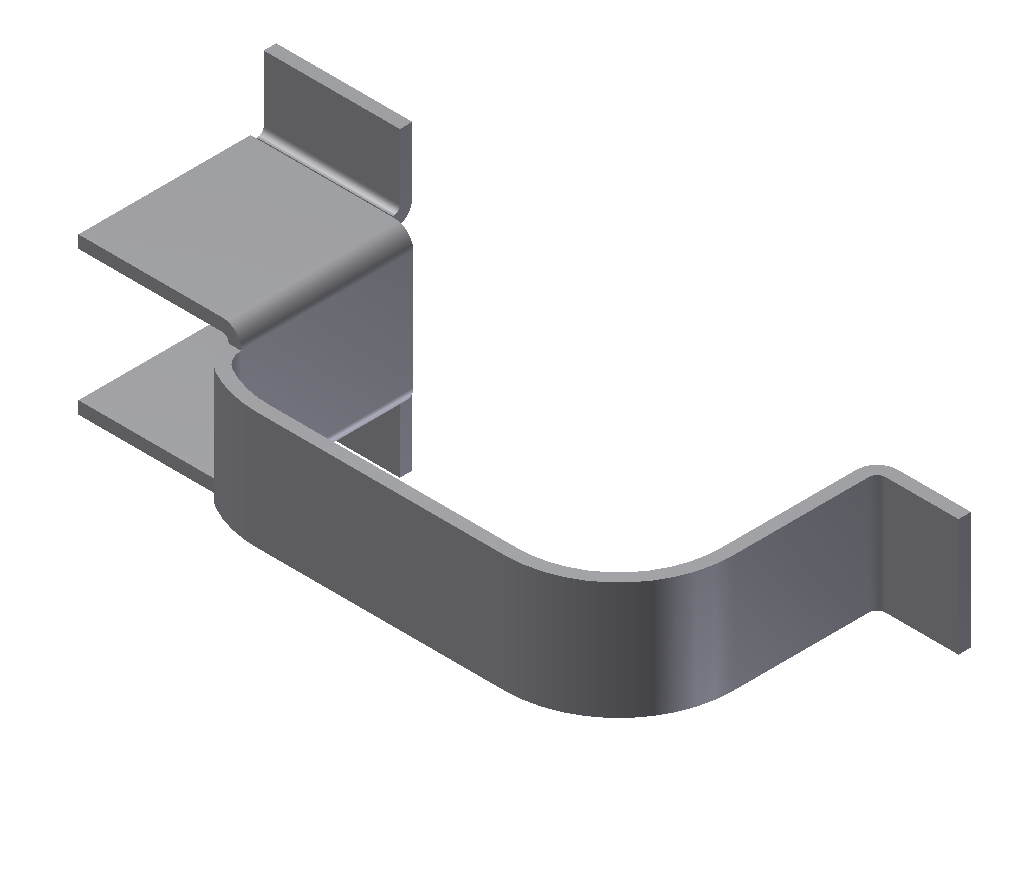
\includegraphics[width=0.98\linewidth]{..//Common/images/ABELBracketOutputPart}} \\ \bottomrule

\end{tabular}
\captionof{figure}{Generalization}\label{fig:abel}
\end{minipage}

\subsection{Midsurface of the Sweep feature} \label{sec:loftmidsurf}

For each Sweep feature, the midsurface patch can be generated in the following manner: 

\begin{itemize}[noitemsep,topsep=2pt,parsep=2pt,partopsep=2pt]

\item  Feature parameters such as {\em profile} and {\em curve} of {\bf $\mathcal{L}$} are extracted.

\item {\bf Midsurface} is computed based on the relative sizes of {\em profile} and {\em curve}.

\begin{itemize}[noitemsep,topsep=2pt,parsep=2pt,partopsep=2pt]

\item {\bf Thin Profile}: If {\em profile} is very small compared to {\em curve} ( $profile_{length} \ll curve_{length}$), then {\em midcurve} (Section \ref{sec:midcurve}) is extracted from the {\em profile} and swept  along the same {\em curve}. This rule is expressed as \loft{}{L}{2}{0, curve, 0 | C_{0,1,2}}{midcurve^{1-n}} 

\item {\bf Midcurve} is a set of {\em curves} lying midway of a 2D {\em profile} and is expressed as 	\generic{\Omega}{M}{}{C}{1}{} {profile} 

%\vspace{-2mm}

\begin{figure}[h]
\centering 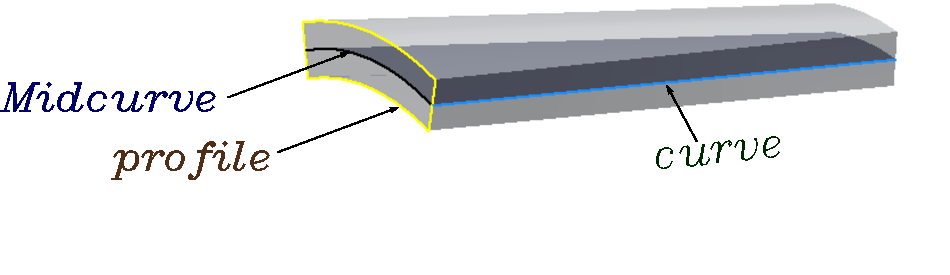
\includegraphics[scale=0.5]{../Common/images//MidsurfSmallProfile_1.pdf} 
%\caption{sketch is far smaller than curve}
\label{figure_MidsurfSmallProfile}
\end{figure}

%\vspace{-9mm}

\end{itemize}

\item {\bf Thin Loft} :  If {\em profile} is very big as compared to {\em curve} ($profile_{length} \gg curve_{length}$), then {\em midcurve} is not extracted  but the {\em profile} itself is {\em swept} along half of the {\em curve}. This rule is expressed as \loft{}{L}{2}{0, curve/2, 0 | C_{0,1,2}}{profile}.
%
%\begin{figure}[htbp]
%\centering 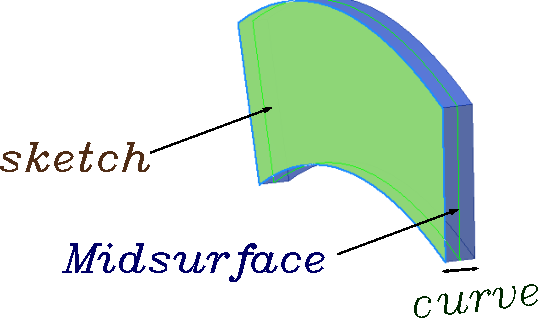
\includegraphics[scale=0.40]{../Common/images//MidsurfSmallCurve.pdf}
%\caption{sketch is far bigger than curve}
%\label{figure_MidsurfSmallCurve}
%\end{figure}

\item {\bf Thick Sketch}:   If {\em sketch} is comparable in size to {\em curve}  ($sketch_{length} \approx curve_{length}$), then it is a thick shape and Midsurface is not generated.

\end{itemize}

\section{Midcurve} \label{sec:midcurve}
Midcurve is set of connected 2D curves lying midway of a 2D profile. As seen before, to generate a midsurface patch of a Thin Profile, midcurve of the profile needs to be computed. This research focuses on 2D planar polygonal sketch profiles with an assumption that curved shapes can be converted to polygonal shape by faceting. In the first  phase of the computation, a  polygon is partitioned into primitive sub-polygons and then in the 2nd phase, midcurve-segments are computed in the non-interface-polygons.  At the end, individual midcurve-segments  are extended-joined to form a continuous set of curves mimicking the parent shape. 

\subsection{Polygon Decomposition}
A polygon can be broken into convex regions by eliminating all reflex vertices. A reflex vertex can only be removed if the diagonal connecting to it is within the range given by extending its neighboring edges; otherwise, its angle is only reduced.

\subsubsection{Preliminaries}

\begin{enumerate}
[noitemsep,topsep=2pt,parsep=2pt,partopsep=2pt,leftmargin=*]
%\begin{list}{}{}
\item {\bf Polygon}: A polygon $P$ of $n$ vertices is defined as $P = \{P_0,P_1,...,P_{n-1}\}$ where, the vertices are in counter clockwise (ccw) order. 

\item {\bf Collinear}: $P_{j+1}$ is {\em Collinear} with $ \overline{P_{j-1} P_j}$ if $Area( P_{j-1}, P_j,  P_{j+1}) = 0$ 

\item {\bf Reflex}: Let  $ P_{j-1}, P_j,  P_{j+1} \in P$ , if the interior $\angle P_{j-1}, P_j,  P_{j+1}$ is greater than $\pi$,  then $P_j$  is a concave or {\em reflex} vertex. $Area < 0$

\item {\bf Intersect}: For  $\overline{P_i P_j}$ to intersect $\overline{P_k P_l}$, either of $P_k, P_l$ should be on the {\em Left} of  $\overline{P_i P_j}$ and the other vertex should be on the {\em Right}. Intersection could be of the {\em Line} type, where extended intersection can be calculated or of  the {\em Segment} type, where only internal (within the range of either of the segments, $\overline{P_i P_j}$ or $\overline{P_k P_l}$) intersections are returned.

\item {\bf Visibility/Can-See}: $P_k$ is visible from $P_i$, if $\overline{P_i P_k}$ is a {\em diagonal} of $P$. 

%\end{list}
\end{enumerate}

\subsubsection{Steps}
Let $P$ be a simple polygon.  The Partitioning of $P$ is defined by the decomposition of $P$ into partitions of non-overlapping sub-polygons by adding internal {\em diagonals} between vertices  $P_i$, or by adding new (Steiner) vertices on {\em edges} $\overline{P_i P_j}$. Partitioning is continued till all possible cuts are made.

\bigskip

\begin{tabular}[h]{@{}p{0.25\linewidth}  p{0.15\linewidth}  p{0.05\linewidth} p{0.25\linewidth}  p{0.15\linewidth}@{}}
%\begin{enumerate}
%[noitemsep,topsep=2pt,parsep=2pt,partopsep=2pt,leftmargin=*]
%\begin{list}{}{}

%------------------------------------------------------------------------------------------------------------------------------------
%\item 
Go through all the vertices of the polygon, one by one in a counter-clockwise manner. Current vertex is called $P_i$ &

\raisebox{-.9\height}{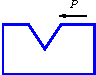
\includegraphics[width=0.8\linewidth]{..//Common/images/polydecomp_traverse.pdf} } & $\Rightarrow$ &

%------------------------------------------------------------------------------------------------------------------------------------
%\item 
Check if $P_i$ is a Reflex vertex $R$ &



\raisebox{-.9\height}{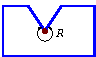
\includegraphics[width=0.8\linewidth]{..//Common/images/polydecomp_reflex.pdf} }\\ \\

%------------------------------------------------------------------------------------------------------------------------------------
%\item 
Extend lines incident at $R = P_i$ (the line coming into $P_i$ and going out of $P_i$) till they intersect remaining of the Polygon, say at $Q_1$ and $Q_2$. Contour within $Q_1$ and $Q_2$ is called $Range$ &

\raisebox{-.9\height}{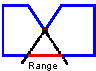
\includegraphics[width=0.8\linewidth]{..//Common/images/polydecomp_range.pdf} }&  $\Rightarrow$ &

%------------------------------------------------------------------------------------------------------------------------------------
%\item 
If there are no $P_i$s within the $Range$ and if any of the $Range$ vertices are close to intersections, separate the triangle out, else, create a new one at the middle on the contour. This newly created point  $Q_m$ is called Steiner point.  $RQ_m$ is the partition-chord to divide the polygon &

\raisebox{-.9\height}{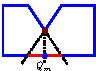
\includegraphics[width=0.8\linewidth]{..//Common/images/polydecomp_mid.pdf} }\\ \\

%------------------------------------------------------------------------------------------------------------------------------------
%\item 
If there are few vertices within the $Range$, choose the best one based on the following priorities:
\begin{enumerate}
[noitemsep,topsep=2pt,parsep=2pt,partopsep=2pt,leftmargin=*]
\item Highest: Closest Reflex
\item Medium: Reflex 
\item Low: Closest 
\end{enumerate} 

& 

\raisebox{-.9\height}{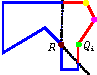
\includegraphics[width=\linewidth]{..//Common/images/polydecomp_choice.pdf} }&  $\Rightarrow$ &
 Make sure that point $Q_i$ is visible from the reflex point $R$. If it is not so, then this cut can not be made. Choose the next best choice. \\ \\

%------------------------------------------------------------------------------------------------------------------------------------
%\item 
Once vertex is chosen, say, $Q_i$, create partition chord $RQ_i$ and divide the  polygon.&

\raisebox{-.9\height}{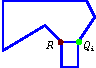
\includegraphics[width=\linewidth]{..//Common/images/polydecomp_divide.pdf} } &  $\Rightarrow$ &


%\end{tabular}

%------------------------------------------------------------------------------------------------------------------------------------
%\item 
Send individual sub-polygons to the same process recursively till there are no reflex vertices left.  \\ \\

%\item  
Identify polygons with more than 4 distinct (ignoring sub-segment overlapping chords) sides. Triangulate them with Constrained Delaunay Triangulation (CDT).&

\raisebox{-.9\height}{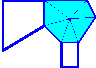
\includegraphics[width=\linewidth]{..//Common/images/polydecomp_divide_all.pdf}}  &  $\Rightarrow$ &

CDT takes care of the remaining relative  areas of the polygon.\\

%\end{list}
%\end{enumerate}
\end{tabular}

\bigskip

This technique improves upon the Bayazit's algorithm \cite{Bayazit} in terms of expanding search to include even extreme vertices in the range, thereby giving minimal and elongated partitions. Midcurves are typically for thin-elongated shapes. This improvement results in the sub-polygons of necessary shape characteristics.

\smallskip

\begin{tabular}[h]{@{}p{0.6\linewidth} p{0.01\linewidth} p{0.27\linewidth}@{}}

If any incoming edge ($MR$) was hitting the end points of the test-line ($QN$) or was collinear, it ($Q$) was getting ignored in the existing algorithm \cite{Bayazit}. In that case, the next closet vertex ($S$) was getting chosen. This was corrected in the proposed algorithm and the shorter cut ($RQ$) is done.&&

\raisebox{-.9\height}{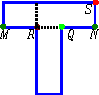
\includegraphics[width=0.45\linewidth]{..//Common/images/polydecomp_mine.pdf} } \\
\end{tabular}

\smallskip

Decomposition helped getting in the sub-polygons which are of primitive shapes and which are easier for Midcurves creation compared to the original-whole shape. 

\subsection{Midcurve Computation}

\begin{tabular}[h]{@{}p{0.28\linewidth}   p{0.05\linewidth} p{0.28\linewidth}  p{0.05\linewidth} p{0.28\linewidth}@{}}
%\begin{enumerate}
%[noitemsep,topsep=2pt,parsep=2pt,partopsep=2pt,leftmargin=*]
%\begin{itemize}
%------------------------------------------------------------------------------------------------------------------------------------
%\item
Each partitioning edge inserted during the decomposition is called as a `chord'. &  $\Rightarrow$ &
Generate Midcurves for individual polygons longer length-wise, on both sides of the `chord'&   $\Rightarrow$ &
When curves do not meet at the chord', extend upto the midcurve. \\ \\

\centering \raisebox{-.9\height}{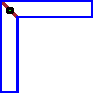
\includegraphics[width=0.36\linewidth]{..//Common/images/midcurve_polydecomp.pdf}} & &
\centering \raisebox{-.9\height}{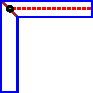
\includegraphics[width=0.36\linewidth]{..//Common/images/midcurve_polymid.pdf}}  & &
\centering  \raisebox{-.9\height}{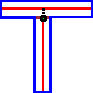
\includegraphics[width=0.36\linewidth]{..//Common/images/midcurve_extend.pdf}} 
\\
%\end{itemize}
\end{tabular}
%\end{enumerate}
%\vspace{.1cm}

\bigskip

This midcurve is used later in the midsurface patch computation (Section \ref{sec:scell}). Following are the sample-profiles taken from past research papers, and along with the midcuves computed from the above-mentioned process.

\bigskip

\begin{tabular}[h]{@{}p{0.28\linewidth} p{0.28\linewidth} p{0.28\linewidth}@{}}
%\begin{enumerate}
%[noitemsep,topsep=2pt,parsep=2pt,partopsep=2pt,leftmargin=*]
%\begin{itemize}
%------------------------------------------------------------------------------------------------------------------------------------
%\item
Glass profile by Fischer \cite{Elber1999}. &
Profile by Ramanathan \cite{Ramanathan2004}. &
Plastic Part profile by Sheen \cite{Sheen2010}. \\ \\

\raisebox{-.9\height}{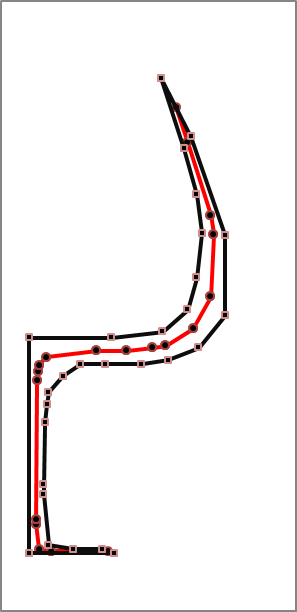
\includegraphics[angle=90, width=0.85\linewidth]{..//Common/images/Glassmc.png}} &
\raisebox{-.9\height}{\includegraphics[width=0.85\linewidth]{..//Common/images/DoubleKmc.png}}  &
\raisebox{-.9\height}{\includegraphics[width=0.85\linewidth]{..//Common/images/Sheen1mc.png}} 
\\
%\end{itemize}
\end{tabular}

\bigskip



\section{Midsurface}
After defeaturing and feature abstraction, the feature tree is then decomposed by feature-based cellular decomposition (FBCD) in which the feature volumes are partitioned into cell-bodies in such a way that there is no volumetric overlap. However, the cells can touch others at the boundary faces ($O$, faces have dimensionality 2, called ``cell-faces'') fully, not partially (Figure \ref{fig_fbcd}). 

\begin{figure}[!h]
\centering     %%% not \center
\subfloat[Original Part]{\label{fig_orig}\includegraphics[width=0.26\linewidth,valign=t]{../Common/images/DecompBracketInput}}
\subfloat[Decomposition]{\label{fig_cd}\includegraphics[width=0.25\linewidth,valign=t]{../Common/images/DecompBracketOutput}}
\subfloat[Before decomposition]{\label{fig_twofeat}\includegraphics[width=0.2\linewidth,valign=t]{../Common/images/FeatureInteractionMergedPart.pdf}} \quad
\subfloat[After decomposition]{\label{fig_featinteract}\includegraphics[width=0.2\linewidth,valign=t]{../Common/images//FeatureInteractionMergedCells.pdf}}
\caption{ Feature-based cellular decomposition}
\label{fig_fbcd}
\end{figure}

Figure \ref{fig_twofeat} shows a representative case, where two features $f_1$ and $f_2$ are interacting. Interaction can have full/partial volumetric/surface overlaps. Decomposition used in this work uses primary rules as follows:
\begin{itemize}[noitemsep,topsep=2pt,parsep=2pt,partopsep=2pt]
\item Booleans (Internal/External) are changed to ``New Body'' type, so that tool-body volumes are decoupled.
\item Faces at concave edges are extended and used as partitions to split the volumes. Extension does not happen indefinites but within the influence zone decided by two interacting features.
\end{itemize}

This FBCD technique scores over some of the past techniques such that, partitioning does not populate too many/redundant cells due to global splitting. It also retains the feature ownerships, so that each cell knows the original Sweep feature to which it belongs and can query the corresponding profile and guide curve.

In the scenario shown above, volumes of $f_1$ and $f_2$ are partitioned in such a way that a common cell (with owner $f''_1f''_2$) is formed (Figure \ref{fig_featinteract}). Remaining portions of $f_1$ and $f_2$ are termed as $f'_1$ and $f'_2$ respectively.  Overlapping faces are denoted as $O_1$ and $O_2$. Thus, now, the cell-bodies do not overlap volumetrically [$O_{i,j}^3$], but may overlap at faces [$O_{i,j}^2$] fully [ $C_i \cap C_j = 0| O_{i,j}^2$].

FBCD results in $n$ cell-bodies with owning-feature(s) assigned to each of them. A cell adjacency graph [CAG, $G(n,e)$] is formed with the $n$ nodes, each representing a cell-body. For each face-overlap between two nodes, an edge ($e$), having two nodes ($n$) attached on either end, is created in the CAG.  Figure \ref{fig_featgraph} shows the CAG of simple cell bodies configuration shown in Figure \ref{fig_fbcd}. Advantage of the CAG representation is that it is easier to classify nodes and delegate specific computational work to them. Actual computation of midsurface geometry is delegated to the nodes having unique owning-feature, where as others are meant to join the midsurface patches. Thus, this research does not need to enumerate specific heuristic rules used for specific connection types.


%\begin{figure}[h]
%\centering 
\begin{minipage}[h]{0.68\linewidth} 
\begin{minipage}[h]{0.4\linewidth} 
\includegraphics[width=0.8\linewidth]{../Common/images/FeatureInteractionGraph.pdf}
\captionof{figure}{Feature Cellular Graph}
\label{fig_featgraph}
\end{minipage}
\hfill
\begin{minipage}[h]{0.4\linewidth} 
\begin{itemize}[noitemsep,topsep=2pt,parsep=2pt,partopsep=2pt,label={}]
\item $n_1 = sCell_1= f'_1$
\item $n_2 = iCell_1 = f''_1f''_2$
\item $n_3 = sCell_2 = f'_2$
\item $e_{12} = O_1$
\item $e_{23}= O_2$
\end{itemize}
\end{minipage}
\end{minipage}
%\end{figure}

Node $n_1$ corresponds to a cell-body, with owning feature $f'_1$, whereas node $n_3$ corresponds to the cell-body with owning feature $f'_2$. The common cell-body owned by $ f''_1f''_2$ is represented by node $n_2$.  Edge $e_{12}$ corresponds to the overlapping face $O_1$, where as  Edge $e_{23}$ corresponds to the overlapping face $O_2$.
Looking at the connectivity at each cell-node, they are classified into solid cells ($sCell$) and interface cells ($iCell$)  %The commonly-shared cells are marked as interface cells ($iCell$) and the others as solid cells ($sCell$)  
This classification strategy simplifies the complexity of the midsurface generation problem to a great extent. Since, generating a midsurface patch for $sCell$  is relatively straight-forward, these are discrete volumes with known owning-feature of only one type, ``Sweep''. For Sweep, the midsurface patch can be computed in a deterministic manner. The problem of resolving interaction amongst the midsurface patches is carried out in the $iCell$s, again in a reliable manner.
%
%\begin{mydef}
%Interface cell ($iCell$) is a node with more than 2 incident edges and has respective overlapping faces ($O_1,O_2$) adjacent to each other.
%\end{mydef}
%\begin{mydef}
%Solid cell ($sCell$) is any adjacent node with owning-feature as ``Sweep'' and is not an $iCell$.
%\end{mydef}
%
%\begin{figure}[h]
%\centering 
%\begin{minipage}[h]{0.48\linewidth} 
%\centering \includegraphics[width=0.4\linewidth]{../Common/images/CellDecompExample.pdf}
%\caption{Classification of Cells (\cite{Treeck})}
%\label{fig_celldecompexample}
%\end{minipage}
%\begin{minipage}[h]{0.48\linewidth} 
%\begin{mydef}
%Interface cell ($iCell$) is a node with more than 2 incident edges and has respective overlapping faces ($O_1,O_2$) adjacent to each other.
%\end{mydef}
%\begin{mydef}
%Solid cell ($sCell$) is any adjacent node with owning-feature as ``Sweep'' and is not an $iCell$.
%\end{mydef}
%\end{minipage}
%\end{figure}
%\bigskip

%\begin{mydef}
%Interface cell ($iCell$) is a node with more than 2 incident edges and has respective overlapping faces ($O_1,O_2$) adjacent to each other.
%\end{mydef}
%
%\begin{mydef}
%Solid cell ($iCell$) is any node which is not an $iCell$.
%\end{mydef}
%
%	\begin{figure} [!h]
%	\centering
%	\includegraphics[width=0.7\linewidth]{../Common/images/CellDecompExample}
%	\caption{Decomposition and Classification of Cells (\cite{Treeck})}
%	\label{fig_celldecompexample}
%	\end{figure}
				
In Figure \ref{fig_featgraph},  $n_1$ and $n_3$ are solid cells ($sCell$), where as $n_2$ is an interaction cell ($iCell$).  $sCell$ are midsurface patch-computing cells, which look at the $profile$ and $guide$ of the owning-feature to compute the midsurface patch. $iCell$ are interaction-resolving cells, connecting all the midsurface patches incident on it. Midsurface computation strategies for $sCell$s and  $iCell$s are detailed out in the sections below.
			
\subsubsection{Computing midsurface patches in $sCell$s}
\label{sec:scell}
The CAG is traversed node by node. The owning-feature corresponding to the cell represented by the current node is extracted. A midsurface patch is computed looking at the feature parameters of owner sweep feature such as the profile $p$ and the guide curve $g$ .% (\cite{YogeshIITG2014}). %%%%%%%%%% ADD (\cite{YogeshIITG2014}) LATER		
Midsurface patches are computed in each $sCell$ as per the methodology as mentioned in Section \ref{sec:loftmidsurf}. Once all the $sCell$s are done with the computation of midsurface patches, the next step is to resolve interactions  between these patches in $iCell$s.

%\begin{mydef}
%\label{def:thinprofile}
%The profile $p$ is considered thin, if its size (characterized by the length of its perimeter) is less than the threshold-factor times the length of the guide curve $g$ (Fig. \ref{fig_ablemids}). Otherwise the profile is considered as ``Thick''.
%\end{mydef}



%Midsurface patches are computed based on following strategies  :%(Fig. \ref{fig_ablemids})  (Algorithm \ref{alg_MidsurfsCell}) :
%%For `Thick Profile' \ref{def:thinprofile}) the profile-face is offset, else (called `Thin Profile', definition \ref{def:thinprofile}) , midcurve of $p$ is swept along $g$ (Figure \ref{fig_ablemids}).
%	\begin{itemize}[noitemsep,topsep=2pt,parsep=2pt,partopsep=2pt]
%	\item \textbf{Strategy 1}:  If the profile $p$ is thin, a midcurve ($m^1$) is computed from $p$ and it  is swept using the guide curve $g$ to generate the midsurface patch $m^2$ %(Fig. \ref{fig_thin}).
%	\item\textbf{Strategy 2}:  If the profile $p$ is thick, $p$ is offset by half of $g$ so as to lie midway to generate the midsurface patch $m^2$  %(Fig. \ref{fig_thick}). 
%	\end{itemize}

%	\begin{figure}[!h]
%	\centering     %%% not \center
%	\subfloat[Sweep feature]{\label{fig_thickthinpart}\includegraphics[width=0.23\linewidth,valign=t]{../Common/images/ThickThinProfilePart}}
%	\subfloat[Thick profile midsurface]{\label{fig_thick}\includegraphics[width=0.23\linewidth,valign=t]{../Common/images/ThickProfileMidsurf}}
%	\subfloat[Thin profile midsurface]{\label{fig_thin}\includegraphics[width=0.23\linewidth,valign=t]{../Common/images/ThinProfileMidsurf}}
%	\subfloat[Midsurface patches]{\label{fig_scells}\includegraphics[width=0.23\linewidth,valign=t]{../Common/images/MidsurfPatches.pdf}}	
%	\caption{Midsurface based on relative size of Profile and Guide curve  (\cite{YogeshIITG2014}) } %%%%%%%% ADD (\{citeYogeshIITG2014}) LATER
%	\label{fig_ablemids}
%	\end{figure}

%Applying these strategies for $sCell$s shown in Figure \ref{fig_fbcd}, the corresponding midsurface-patches generated are as shown in Figure \ref{fig_scells}. 
%	
%\begin{figure}[!h]
%\centering 
%\begin{minipage}[h]{0.4\linewidth} 
%\includegraphics[width=0.7\linewidth]{../Common/images/MidsurfPatches.pdf}
%\caption{Midsurface patches of two $sCell$s}
%\label{fig_scells}
%\end{minipage}
%\begin{minipage}[h]{0.58\linewidth} 
%Rules for computing midsurface patch are:
%	\begin{itemize}[noitemsep,topsep=2pt,parsep=2pt,partopsep=2pt]
%	\item \textbf{Rule 1}:  If the profile $p$ is thin, a midcurve ($m^1$) is computed from $p$ and it  is swept using the guide curve $g$ to generate the midsurface patch $m^2$ (Fig. \ref{fig_thin}).
%	\item\textbf{Rule 2}:  If the profile $p$ is thick, $p$ is offset by half of $g$ so as to lie midway (Fig. \ref{fig_thick}). 
%	\end{itemize}
%	After computation of the midsurface patches, scenario shown in Figure \ref{fig_fbcd} results as in Figure \ref{fig_scells}.
%\end{minipage}
%\end{figure}

%	
%	\begin{algorithm}[!h]
%		\caption{sCell midsurface patch computation}
%		\label{alg_MidsurfsCell}
%		\begin{algorithmic}
%			\REQUIRE $sCell$
%			\ENSURE $size(sCell \rightarrow owning-feature(s)) = 1$
%			\STATE $f = sCell \rightarrow owning\_feature()$
%			\STATE $p = f \rightarrow get\_profile()$
%			\STATE $g = f \rightarrow get\_guide\_curve()$
%			%\STATE $is\_thin\_profile = \sqrt{Area(profile)} < threshold \times length(guide)$ 
%			\IF{$is\_thin\_profile(p) == true$}
%				\STATE $m^1 = p\rightarrow compute\_midcurve()$
%				\STATE $m^2 = sweep(m^1 ,g)$
%			\ELSE
%				\STATE $m^2 = offset(p ,g/2)$
%			\ENDIF
%		\end{algorithmic}
%	\end{algorithm}
	
	



\subsubsection{Resolving interactions between midsurface patches in $iCell$s}
\label{sec:icell}
Input to this module is a CAG with midsurface patches computed at all the $sCell$s. The sole responsibility of $iCell$s is to connect the midsurface patches incident on them, either by extending the midsurface-patches from the adjacent $sCell$s or by generating new ones.  The CAG is used to traverse $iCell$s one by one. For each $iCell$, the midsurface patch interactions are resolved as follows:
%\vspace{-3mm}
	\begin{figure}[!h]
	\centering     %%% not \center
	\subfloat[Expected adjustments]{\label{fig_icells}\includegraphics[width=0.25\linewidth,valign=t]{../Common/images/MidsurfJoining.pdf}}
	\subfloat[$sCell-iCell$ scenario]{\label{fig_sextensions}\includegraphics[width=0.25\linewidth,valign=t]{../Common/images/sCellExtension.pdf}}
	\subfloat[$iCell-iCell$ scenario]{\label{fig_iextensions}\includegraphics[width=0.25\linewidth,valign=t]{../Common/images/iCellExtension.pdf}}	
	\caption{Resolving Interactions in the $iCell$}
	\label{fig_resolveiCell}
	\end{figure}
%\vspace{-2mm}
%\bigskip
%	
%	\begin{algorithm}[!h]
%		\caption{$iCell$ midsurface patch interaction resolution}
%		\label{alg_MidsurfiCell}
%		\begin{algorithmic}
%			\REQUIRE $iCell$
%			\WHILE{$size(iCell \rightarrow edges) > 0$}
%				\STATE $e_i = iCell \rightarrow edge$
%				\STATE $n_s = iCell $	
%				\STATE $n_o = e_i \rightarrow get\_adjacent\_node(n_s) $			
%				\IF{$n_o \rightarrow type == sCell$}
%					\STATE $m_o = n_o \rightarrow query\_midsurface()$
%					\STATE $O_f = e_i \rightarrow overlapping\_face()$
%					\STATE $m^1 = surf\_surf\_intersection(O_f, m_o)$
%					\STATE $m^2 = extrude(m^1, n_o \rightarrow centroid)$
%				\ELSIF{$n_o \rightarrow type == iCell$}
%					\STATE $c^1_1= get\_curve\_at\_centroid(n_s)$
%					\STATE $c^1_2 = get\_curve\_at\_centroid(n_o)$
%					\STATE $m^2 = create\_patch(c^1_1, c^1_2)$
%					\ENDIF
%			\ENDWHILE
%		\end{algorithmic}
%	\end{algorithm}
%
%\bigskip
Each $iCell$ is connected with adjacent cells via edges $e$(s).  Each incident $e$ has two nodes (as $e_{12}$ has $n_1$ and $n_2$  in Figure \ref{fig_featgraph} ), where one is the ``self'', the current $iCell$ and the second one is called the ``adjacent node''.  The ``adjacent node'' could be either a $sCell$ or an $iCell$.  

If the ``adjacent node'' is a $sCell$, the adjacent midsurface-patch is extended up to $iCell$'s centroid (Fig. \ref{fig_sextensions}). An intersection curve ($m^1$) is computed between the overlapping face ($O_{1,2}$) and the midsurface ($m^2$). This curve acts as a midcurve for the extension into the $iCell$. In case, where all the three cells are geometrically flat and relatively big, then all are marked as  $sCell$s (not $iCell$s) and have no extensions. 

If the ``adjacent node'' is an $iCell(n_3)$, an extra patch is created between the centroids of the two $iCell$s (Fig. \ref{fig_iextensions}). Thus, all the $iCell$s join the midsurface patches (Fig. \ref{fig_icells}) to form a well-connected midsurface.

%
%The overall algorithm for computing the midsurface leveraging FBCD is presented in Algorithm \ref{alg_FBDMidsurf}.
%
%\bigskip
%
%\begin{algorithm}[!h]
%\caption{Feature-based midsurface computation}
%\label{alg_FBDMidsurf}
%\begin{algorithmic}
%	\REQUIRE Feature-based CAD model  represented by  ($\cup_mf^3$)
%	\STATE $\cup_nf^3 = feature\_based\_defeaturing(\cup_mf^3)$, where, $n \leq m$
%	\STATE $\cup_nL^3 = feature\_based\_generalization(\cup_nf^3 )$
%	\STATE $\cup_uC^3 =feature\_based\_cellular\_decomposition(\cup_nL^3)$, where, $C_i \cap C_j = 0| O_{i,j}^2$
%	\STATE $G(n, ) = compute\_graph\_nodes(\cup_uC^3)$
%	\STATE $(Gn,e) = find\_overlaps\_generate\_edges(G(n, ))$
%	\STATE $(sCell,iCell) = categorize\_cells((Gn,e))$
%%	\IF{ $n_i\rightarrow edges > 2$ \& \ $n_i \rightarrow body \rightarrow is\_thin = true$ \& $O_{i,j}^2$ are adjacent} 
%%		\STATE $type(n_i) = iCell$ 
%%	\ELSE
%%		\STATE $type(n_i) = sCell$
%%	\ENDIF
%	\FORALL{$sCell$}
%		\STATE $\cup_vL^2 = compute\_midsurface\_patch(sCell)$ (Algorithm \ref{alg_MidsurfsCell})
%	\ENDFOR
%	\FORALL{$iCell$}
%		\STATE $\cup_wL^2 = resolve\_interactions(iCell)$ (Algorithm \ref{alg_MidsurfiCell})
%	\ENDFOR
%	\RETURN $\cup_uL^2 = (\cup_vL^2) \cup (\cup_wL^2)$
%
%\end{algorithmic}
%\end{algorithm}

Once all interactions are resolved in $iCell$s, the result is a well-connected midsurface. Cached dormant bodies are pierced into the midsurface  (Section \ref{sec:dormant}) to restore the temporarily-suppressed  negative features (Figure \ref{fig_midsdorm}).

%\vspace{-8mm}

	\begin{figure}[!h]
	\centering     %%% not \center
%	\subfloat[Original Part]{\label{fig_origpart}\includegraphics[width=0.3\linewidth,valign=t]{../Common/images/DefeatBracketPhase_I_1}} \quad
	\subfloat[Dormant Bodies piercing]{\label{fig_midsdorm}\includegraphics[width=0.3\linewidth,valign=t]{../Common/images/MidsurfDormantBodies}} \qquad
	\subfloat[Final Output]{\label{fig_finalmids}\includegraphics[width=0.3\linewidth,valign=t]{../Common/images/MidsurfAfterDormant}}	
	\caption{Computation of Midsurface of a Bracket}
	\label{fig_midsdorm}
	\end{figure}
	
%\vspace{-2mm}

The superiority of the proposed approach is in the manner in which it has abstracted both the sub-problems, i.e., computation of midsurface patches and resolving interactions amongst them. No heuristic rules based on specific surface-types or connection configurations are used, making the whole process generic and adaptable in a wide variety of configurations.

%\section{Results}
%\label{results}
%
%The algorithms presented here have been implemented using the  Autodesk\textsuperscript{\textregistered} Inventor's Application Programming Interface (API) in Visual Basic.Net.  Following are the results of some sample test cases run on an Intel i3 64-bit 2 GHz Windows 7 machine (Figure \ref{fig_mids}):


	
%\vspace{-4mm}
%\begin{figure}[!h]
%\centering     %%% not \center
%\includegraphics[width=0.3\linewidth,valign=t]{../Common/images/DefeatBracketPhase_I_1} \quad
%\includegraphics[width=0.3\linewidth,valign=t]{../Common/images/MidsurfBracket} \quad
%\includegraphics[width=0.3\linewidth,valign=t]{../Common/images/MidsurfBracket}
%\caption{Computation of Midsurface of a Bracket}
%\label{fig_mids}
%\end{figure}
%\vspace{-4mm}

\section{Validation}
\label{Validation}

Midsurface is expected to truly represent the original solid, both in terms of geometry and topology. It is tedious to follow the manual process of inspection to validate it, especially for the complex models. The present system performs such validation in an automated way and uses Hausdorff's distance measure to verify geometric correctness. However, as a necessary and sufficient validation, the system also carries out topological validation to verify the connectivity as well as missing surfaces or gaps. The following section demonstrates the formulation developed to carry out such validation.% (\cite{YogeshCADandA2015}). 

The main idea behind the formulation is that, the generated midsurface is expected to be such that it is obtained as if the solid body is shrunk to its overall neutral plane. As a reverse validation, if such a midsurface is thickened it should represent a solid body as close to the original solid as possible. The solid's topological validity is then checked using Euler-Poincar\'e's manifold equation. If the original midsurface had any gaps or overlaps, the resultant solid will not satisfy the manifold condition. 

Procedure to validate midsurface is as follows:% (\cite{YogeshCADandA2015}):   %%%%%%%%%%% ADD in (\cite{YogeshCADandA2015}) LATER

\begin{figure}[h]
\centering 
\begin{minipage}[h]{0.5\linewidth} 
\includegraphics[width=\linewidth]{../Common/images/NonManifoldT1.pdf}
\captionof{figure}{Non-Manifold topological entities}
\label{fig_nonmanifold}
\end{minipage}
\begin{minipage}[h]{0.45\linewidth} 
Steps:
\begin{enumerate}[noitemsep,topsep=2pt,parsep=2pt,partopsep=2pt]
\item Classify Midsurface entities  as : $f, e_s , e_{sr} , e_{rr}, e_r , e_i, v_s , v_r , v_i, s , h , r$ (Figure \ref{fig_nonmanifold}).
\item Predict topological entities using the equations developed. % (\cite{YogeshCADandA2015})%%%%%%%%% ADD  in (\cite{YogeshCADandA2015}) LATER
%\item Verify that the topological entities of the Midsurface satisfy the non-manifold equation, by showing that left ($\chi_{nml}$) and right  ($\chi_{nmr}$) hand side of the equation matches.
\item Verify that the predicted topological entities of the  thin-walled solid satisfy the manifold equation by showing that left ($\chi_{ml}$) and right  ($\chi_{mr}$) hand side of the equation matches. %Thus proving that the transformation equations are valid. 
\end{enumerate}
\end{minipage}

\end{figure}





\begin{tabular}[htp]{@{}p{0.48\linewidth}  p{0.48\linewidth}@{}} \toprule
{\bf Midsurface} & {\bf Edge Classification} \\ \midrule
\includegraphics[width=0.6\linewidth]{../Common/images/SimpleBracketMidsurfshaded.pdf} &
\includegraphics[width=0.6\linewidth]{../Common/images/SimpleBracketMidsurf.pdf}\\ \bottomrule
\end{tabular}

\begin{enumerate}
[noitemsep,topsep=2pt,parsep=2pt,partopsep=2pt]
\item \textbf{Midsurface entities}: \\$f = 15, e_s = 3, e_{sr} = 10, e_r = 14, e_{rr} = 19, l_p = 9 ,e_i=5,v_s = 8,v_r =24, v_i= 5, s=1,h=5,r=5$
\item \textbf{Predicted solid-faces}: \\$f_m = 2f+e_s+ l_p +e_i $\\$= 2 \times 15 + 3 + 9 + 5 = 47$
\item \textbf{Predicted solid-edges}: \\ $e_m = 2(e_s+e_{sr}+e_{rr}+e_i )+ \sum n_{r} e_{r}+v_s+v_i $\\$= 2(3+10+19 + 5)+ (2\times 12 + 4 \times 2)+8+5 = 119$
\item \textbf{Predicted solid-vertices}: \\$v_m = 2(v_s+ v_i) + \sum n_{r} v_r$\\$=2\times (8 + 5)  + 2 \times 24=74$
\item \textbf{Predicted solid-shells-holes}: \\$s_m =s = 1, h_m = r_i  = 5, r_m = 2r_i = 10$
%\item \textbf{Non-manifold equation of the left side}:  $\chi_{nml} $\\$= v-e+f $\\$= 32-46+15 = 1$
%\item \textbf{Non-manifold equation of the  right side}:  $\chi_{nmr}$\\$=s-h+r$\\$=1-5+5 = 1$
\item \textbf{Manifold equation of the  left side}:  $\chi_{ml} $\\$= v_m-e_m+f_m $\\$=74-119+47= 2$
\item \textbf{Manifold equation of the  right side}:  $\chi_{mr}$\\$=2(s_m-h_m )+r_m$\\$= 2(1-5)+10 = 2$
%\item Sheet metal midsurface characteristic $\chi_{smm}$\\$=
%e_s+e_i+(2-n_{r} ) e_{r}+e_{sr}/n_{r} $\\$=v_s+(2-n_{r} ) v_{r}+v_i$\\$ 4+0+0+0=4+0+0= 4$
%\item \textbf{Result}: \textcolor{green}{Matches}
\end{enumerate}
It can be observed that the predicted solid entities validate the manifold equation ($\chi_{ml} = \chi_{mr} = 2$) and the topological entities of the thin-walled solid match with the predicted ones.



